\chapter{The Electron Gun of FLUTE its Stability}
\Gls{flute} is a \gls{linac} based terahertz (THz) photon source currently under commission aiming to be a source of high field THz pulses, provide a test facility for accelerator research and an injection device for \gls{cstart} (see \cite{SchaeferHaererPapash2019_1000091183}) in the future. \cite{Naknaimueang:2011zz}

\begin{figure}[tb]
	\centering
	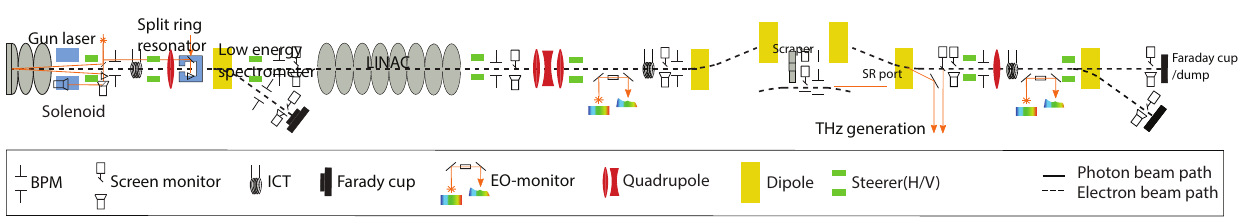
\includegraphics[width=\textwidth]{chap/StabilityOfTheElectronGun/img/flutePaper.png}
	\caption{Schematic of the finished accelerator showing all installed and planned components \cite{Yan2018}}
	\label{fig:fluteEgun-flutePaper}
\end{figure}


\section{The Electron Gun}

\begin{figure}[tb]
	\centering
	\includegraphics[]{chap/StabilityOfTheElectronGun/img/fluteSchem.tikz}
	\caption{}
	\label{fig:fluteEgun-rfschematic}
\end{figure}

\begin{figure}[tb]
	\centering
	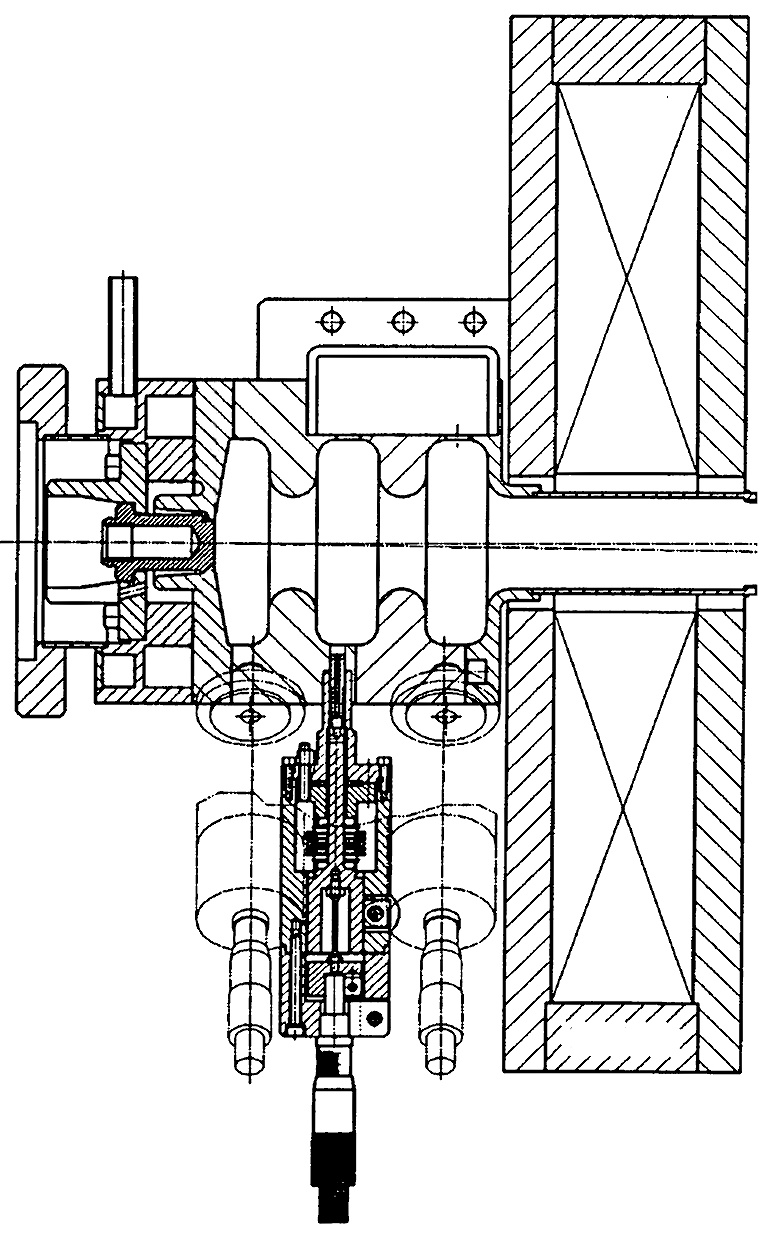
\includegraphics[]{chap/StabilityOfTheElectronGun/img/gun.tikz}
	\caption{Cross section drawing of the electron gun together with the solenoid showing the photo-cathode (red) and the electron and laser beam trajectories
	\\(modified from \cite{Bossart:clic} and \cite{Bossart:288412})}
	\label{fig:fluteEgun-gunDraw}
\end{figure}

\begin{figure}[tb]
	\centering
	\includegraphics[width=\textwidth,height=0.5\textwidth]{chap/StabilityOfTheElectronGun/img/Ez.tikz}
	\caption{Plot of the electrical field in $z$ direction over the length of the gun cavity (redrawn from \cite{Bossart:clic} using geometrical measurements from \cite{Hoeninger2014})}
	\label{fig:fluteEgun-Ezplot}
\end{figure}

\section{Energy Stability of the Emitted Electrons}

\section{Metrics to quantify stability}\label{sec:metrics}
``Stability'' can have different meanings depending on the context. In case of signal processing, a signal is usually said to be \textit{stable} if it has only little variation around its mean or some target value, i.e. the mean has to be constant and the variance stays below some threshold. 
Stability is not to be confused with stationarity, which requires the mean and the variance and the autocorrelation stay constant over time \cite{Guthrie2020}. To express stability as a single numerical value, there are several possibilities, some are described in the following.

\paragraph{Relative Standard Deviation}
This measures the stability as the standard deviation but related to the mean value to make it comparable to other quantities with different scaling or units.

The relative, or percentual, standard deviation of the stationary stoachastic process $X$ is defined using the mean $\mu_X$ and the standard deviation $\sigma_X$ as
\begin{equation}
\op{\%STD_X} := \frac{\sigma_X}{\mu_X}.
\end{equation}
Is the process $X$ non stationary, $\op{\%STD_X}$ depends on the absolute time $t$ and the window size $T$ for which the process is assumed to be stationary:
\begin{equation}
\op{\%STD_X} = \op{\%STD_X}(t,T)
\end{equation}
In that case, for a fixed window size $T=T_0$, a mean percentual standard deviation can be computed with (assuming discrete time steps $t_n$, $n\in[0,N-1]$)
\begin{equation}
\op{\%STD_X}(T=T_0) = \frac{1}{N} \sum_{n=0}^{N-1} \op{\%STD_X}(t_n,T_0)
\end{equation}

\paragraph{Mean Squared Error}
The mean squared error sums up the squared errors $\left(x[n] - x_t[n]\right)^2$ of $x[n]$ from a set value $x_t[n]$. To remove the effect of the length of the data sequence, the sum is devided by the length of the sequence $N$:
\begin{equation}
MSE_x := \frac{1}{N} \sum_{n=0}^{N-1} \left(x[n] - x_t[n]\right)^2
\end{equation}

\paragraph{Relative Power of Most Prominent Noise}
This novel approach compares the power of the most prominent noise power source $P_{noise,\,max}$ of the signal $x$ with the total power $P_x$:
\begin{equation}
MPN_x := \frac{P_{noise,\,max}}{P_x}
\end{equation}



